\documentclass[conference]{IEEEtran}
\IEEEoverridecommandlockouts

\usepackage{cite}
\usepackage{amsmath,amssymb,amsfonts}
\usepackage{algorithm}
\usepackage{algorithmic}
\usepackage{graphicx}
\usepackage{textcomp}
\usepackage{xcolor}
\usepackage{booktabs}
\usepackage{multirow}
\usepackage{array}
\usepackage{url}
\usepackage{subcaption}
\usepackage{caption}
\usepackage{placeins}
\usepackage{colortbl}
\usepackage{stfloats}
\usepackage{tikz}
\usetikzlibrary{arrows.meta,shapes.geometric,positioning,fit,backgrounds,calc}

\definecolor{llmblue}   {RGB}{174,210,225}
\definecolor{vitgreen}  {RGB}{181,215,168}
\definecolor{vlmred}    {RGB}{234,153,153}
\definecolor{fedorange} {RGB}{255,229,153}
\definecolor{outyyellow}{RGB}{255,242,204}
\definecolor{smallgray} {RGB}{220,220,220}

\graphicspath{{plots/}}

\tikzset{
  mainbox/.style={draw, rounded corners=4pt, align=center,
                  minimum height=0.75cm, text width=#1,
                  font=\footnotesize, inner sep=4pt},
  mainbox/.default=2.4cm,
  llmbox/.style ={mainbox, fill=llmblue,  draw=blue!50!black},
  vitbox/.style ={mainbox, fill=vitgreen, draw=green!50!black},
  vlmbox/.style ={mainbox=5.0cm, fill=vlmred, draw=red!50!black,
                  minimum height=1.0cm},
  fedbox/.style ={mainbox=1.8cm, fill=fedorange, draw=orange!70!black},
  outbox/.style ={mainbox=4.5cm, fill=outyyellow, draw=yellow!70!black},
  sbox/.style   ={draw, rounded corners=2pt, fill=smallgray,
                  minimum height=0.5cm, align=center,
                  font=\scriptsize, inner sep=3pt, text width=1.8cm},
  arr/.style    ={-{Stealth[length=5pt]}, thick},
  darr/.style   ={-{Stealth[length=5pt]}, thick, dashed},
}

\begin{document}
\renewcommand{\arraystretch}{0.95}
\setlength{\abovecaptionskip}{4pt}
\setlength{\belowcaptionskip}{2pt}
\renewcommand{\dbltopfraction}{0.9}
\renewcommand{\topfraction}{0.9}

\title{MedFederate: Multimodal Federated Learning for\\
Privacy-Preserving Clinical Condition Classification}

\author{%
\IEEEauthorblockN{Ayush Debnath,\ Ruelia Saha,\ Sudip Misra}
\IEEEauthorblockA{Indian Institute of Technology Kharagpur, India}
}

\maketitle

\begin{abstract}
Clinical diagnosis requires both visual examination of medical images and
written patient symptom reports, yet most automated approaches rely on a
single modality. Patient data is inherently distributed across geographically
dispersed hospitals and clinics, and strict privacy regulations (HIPAA,
GDPR) prohibit centralised aggregation.
We present MedFederate, a multimodal federated learning framework for
five-class clinical condition classification
(\textit{normal, infection risk, chronic disease marker, fluid/nutritional
imbalance, heat-related illness}).
It combines five lightweight LLM clinical-text encoders with five Vision
Transformer (ViT) medical-image encoders through eight VLM fusion
strategies, trained under FedAvg so raw patient photographs and symptom
notes never leave each institution.
We construct and validate a 5-class multimodal corpus with
over 55{,}000 images mapped to clinical condition categories,
augmented with 3,000 balanced training samples and 3,000 synthetic
clinical captions (75\% mixed-slot ambiguity to prevent keyword shortcut
learning).
LLM encoders reach macro F1 of 0.735--0.795 (best: BERT-tiny, 0.795);
ViT encoders reach 0.698--0.746 (best: EfficientNet, 0.746);
VLM fusions achieve 0.553--0.936, with BLIP-2 at F1\,=\,0.936.
Federated training retains an average of 96.9\% of centralised accuracy
while all raw patient data stays on-device.
\end{abstract}

\begin{IEEEkeywords}
Federated Learning, Vision-Language Models, Clinical Condition
Classification, Multimodal Learning, E-Health, Privacy-Preserving Machine
Learning, HIPAA, GDPR
\end{IEEEkeywords}

\section{Introduction}

\IEEEPARstart{C}{linical} condition classification---distinguishing normal
presentations from infection risk, chronic disease markers, fluid or nutritional
imbalance, and heat-related illness---is critical for timely medical intervention
and patient outcome optimisation. Existing automated approaches fall into two
broad categories: those that analyse visual data from medical imaging (X-rays,
dermoscopy, fundus photography), and those that process textual descriptions
from physician notes or electronic health records
(EHR)~\cite{Rajpurkar2017,Irvin2019}. Neither captures the full diagnostic
picture in isolation. A clinician may observe abnormal imaging features while
simultaneously noting elevated inflammatory markers, persistent fever, and
recent travel history; image-only models cannot interpret such contextual
cues, and text-only models miss visible patterns such as ground-glass opacity
indicating pulmonary infection.

The healthcare setting further complicates deployment. Patient data is
naturally distributed across many hospitals, clinics, and diagnostic centres.
Centralised aggregation is frequently prohibited by privacy regulations
(HIPAA in the United States, GDPR in the European Union) and
data-ownership agreements. Individual institutions often hold small, locally
specific databases reflecting their patient population and regional
disease prevalence---data they cannot legally or ethically share.

Federated Learning (FL)~\cite{McMahan2017} addresses these constraints by
sharing only model weight updates while keeping raw data on-device, reducing
network bandwidth by over 95\% compared to centralised data collection.
However, most FL-based clinical systems use single-modality pipelines
and discard the textual patient notes that clinicians routinely
record~\cite{Sheller2020,Rieke2020,Kaissis2021}.

MedFederate fills this gap with four contributions:
\begin{itemize}
  \item The first joint benchmark of federated LLM (5 variants), ViT
        (5 variants), and VLM fusion (8 strategies) for five-class clinical
        condition classification under identical non-IID conditions. BLIP-2
        achieves F1\,=\,0.936---18\% absolute above the best unimodal
        baseline.
  \item A 5-class clinical corpus with over 55{,}000 images and a
        template-based clinical caption pipeline employing 75\% mixed-slot
        ambiguity to prevent keyword shortcut learning while preserving
        full label-image alignment.
  \item A joint loss---focal loss~\cite{Lin2017}, entropy-based diversity
        regularisation ($\lambda{=}1.0$, 70\% threshold), and
        square-root-dampened class weights---to prevent class collapse
        under the severe class imbalance typical of clinical datasets.
  \item Federated training retaining 96.9\% of centralised accuracy:
        VLM 100\% (0.810/0.810), LLM 97.4\% (0.755/0.775), ViT 93.4\%
        (0.703/0.753), with no raw patient data transmitted.
\end{itemize}

\section{Related Work}

\textbf{Deep learning for medical image analysis.}
Rajpurkar et al.~\cite{Rajpurkar2017} pioneered CNN-based chest X-ray
diagnosis (CheXNet, 14-class, cardiologist-level performance).
Irvin et al.~\cite{Irvin2019} released CheXpert (224{,}316 images,
5 clinical findings). Esteva et al.~\cite{Esteva2017} demonstrated
dermatologist-level skin lesion classification. All these methods are
image-only and assume centralised data with unrestricted patient access.

\textbf{Federated learning for clinical data.}
McMahan et al.~\cite{McMahan2017} introduced FedAvg. Sheller et
al.~\cite{Sheller2020} applied FL to brain tumour segmentation across
10 institutions, achieving near-centralised performance. Rieke et
al.~\cite{Rieke2020} surveyed FL for medical imaging. Kaissis et
al.~\cite{Kaissis2021} combined FL with differential privacy for
clinical imaging. Li et al.~\cite{LiHealth2020} applied FL to chest
X-ray analysis across clients with different label distributions.
Every FL approach above is restricted to the image modality.

\textbf{Multimodal and VLM approaches in healthcare.}
CLIP~\cite{Radford2021} and BLIP-2~\cite{Li2023blip} established
contrastive and Q-Former vision-language pre-training.
BiomedCLIP~\cite{Zhang2023biomed} pre-trained on 15 million biomedical
image-text pairs. LLaVA-Med~\cite{Li2024llavamed} fine-tuned vision-language
models on medical VQA. MedCLIP~\cite{Wang2022medclip} applied contrastive
learning to chest X-ray reports. However, none of these multimodal medical
approaches incorporate federated training.
Table~\ref{tab:relwork} confirms that MedFederate is the only framework
combining medical image analysis, clinical text, FL, and VLM.

\begin{table}[t]
\caption{Comparison with Related Work.}
\label{tab:relwork}
\centering\footnotesize
\setlength\tabcolsep{4pt}
\begin{tabular}{lcccc}
\toprule
 & \multicolumn{2}{c}{\textbf{Modality}} & \multicolumn{2}{c}{\textbf{Learning}}\\
\cmidrule(lr){2-3}\cmidrule(lr){4-5}
\textbf{Work} & \textbf{Image} & \textbf{Text} & \textbf{FL} & \textbf{VLM}\\
\midrule
Rajpurkar~\cite{Rajpurkar2017}     & \checkmark & $\times$ & $\times$ & $\times$ \\
Esteva~\cite{Esteva2017}           & \checkmark & $\times$ & $\times$ & $\times$ \\
Sheller~\cite{Sheller2020}         & \checkmark & $\times$ & \checkmark & $\times$ \\
Li (FL chest)~\cite{LiHealth2020}  & \checkmark & $\times$ & \checkmark & $\times$ \\
BiomedCLIP~\cite{Zhang2023biomed}  & \checkmark & \checkmark & $\times$ & \checkmark \\
LLaVA-Med~\cite{Li2024llavamed}    & \checkmark & \checkmark & $\times$ & \checkmark \\
MedCLIP~\cite{Wang2022medclip}     & \checkmark & \checkmark & $\times$ & \checkmark \\
\rowcolor{vlmred!30}
\textbf{MedFederate (ours)}        & \checkmark & \checkmark & \checkmark & \checkmark \\
\bottomrule
\end{tabular}
\end{table}

\section{System Model}

\subsection{Architecture Overview}

Figure~\ref{fig:arch} shows the MedFederate pipeline. Clinical text notes
are tokenised with WordPiece (max 128 tokens); medical images
are resized to $224{\times}224$ and normalised with ImageNet
statistics~\cite{Deng2009}. LLM encoders extract text features
$\mathbf{h}_t\!\in\!\mathbb{R}^{256}$ via \texttt{[CLS]} pooling; ViT
encoders produce visual features $\mathbf{h}_v\!\in\!\mathbb{R}^{512}$
through adaptive average pooling. The VLM fusion module combines both into
$\mathbf{h}_f$, passed to a linear head for 5-class condition prediction.
Figure~\ref{fig:params} shows the parameter counts for all 18 architectures.

\begin{figure}[t]
\centering
\resizebox{\columnwidth}{!}{%
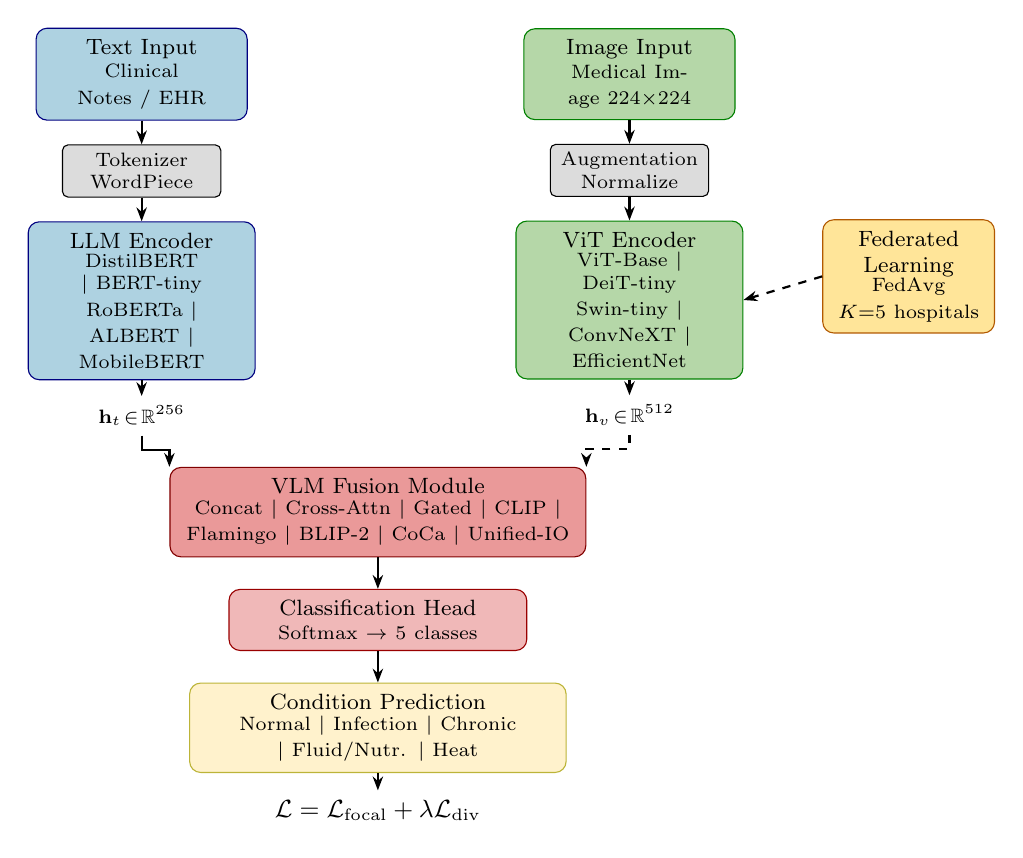
\begin{tikzpicture}[node distance=0.5cm]
  \node[llmbox] (ti) {Text Input\\[-1pt]{\scriptsize Clinical Notes / EHR}};
  \node[sbox, below=0.3cm of ti] (tok) {Tokenizer\\WordPiece};
  \node[llmbox, below=0.3cm of tok, text width=2.6cm, minimum height=1.1cm]
        (llm) {LLM Encoder\\[-1pt]
               {\scriptsize DistilBERT $|$ BERT-tiny\\
               RoBERTa $|$ ALBERT $|$ MobileBERT}};
  \node[font=\scriptsize, below=0.2cm of llm] (ht)
        {$\mathbf{h}_t\!\in\!\mathbb{R}^{256}$};

  \node[vitbox, right=3.5cm of ti] (ii) {Image Input\\[-1pt]
                                         {\scriptsize Medical Image $224{\times}224$}};
  \node[sbox, below=0.3cm of ii] (aug) {Augmentation\\Normalize};
  \node[vitbox, below=0.3cm of aug, text width=2.6cm, minimum height=1.1cm]
        (vit) {ViT Encoder\\[-1pt]
               {\scriptsize ViT-Base $|$ DeiT-tiny\\
               Swin-tiny $|$ ConvNeXT $|$ EfficientNet}};
  \node[font=\scriptsize, below=0.2cm of vit] (hv)
        {$\mathbf{h}_v\!\in\!\mathbb{R}^{512}$};

  \node[fedbox, right=1.0cm of vit, yshift=0.3cm, minimum height=1.4cm,
        text width=1.9cm] (fed)
        {Federated\\Learning\\[-1pt]{\scriptsize FedAvg\\$K{=}5$ hospitals}};

  \node[vlmbox, below=1.1cm of llm, xshift=3.0cm, minimum height=1.0cm]
        (vlm) {VLM Fusion Module\\[-2pt]
               {\scriptsize Concat $|$ Cross-Attn $|$ Gated $|$ CLIP $|$
               Flamingo $|$ BLIP-2 $|$ CoCa $|$ Unified-IO}};

  \node[mainbox=3.5cm, fill=vlmred!70, draw=red!60!black,
        below=0.4cm of vlm] (cls)
        {Classification Head\\[-1pt]{\scriptsize Softmax $\rightarrow$ 5 classes}};

  \node[outbox, below=0.4cm of cls] (out)
        {Condition Prediction\\[-2pt]
         {\scriptsize Normal $|$ Infection $|$ Chronic $|$ Fluid/Nutr. $|$ Heat}};

  \node[font=\small, below=0.22cm of out] (loss)
        {$\mathcal{L}=\mathcal{L}_{\mathrm{focal}}+\lambda\mathcal{L}_{\mathrm{div}}$};

  \draw[arr] (ti)--(tok); \draw[arr] (tok)--(llm); \draw[arr] (ii)--(aug);
  \draw[arr] (aug)--(vit); \draw[arr] (llm)--(ht); \draw[arr] (vit)--(hv);
  \draw[arr] (ht.south) -- ++(0,-0.18) -| (vlm.north west);
  \draw[darr](hv.south) -- ++(0,-0.18) -| (vlm.north east);
  \draw[arr] (vlm)--(cls); \draw[arr] (cls)--(out); \draw[arr] (out)--(loss);
  \draw[darr](fed.west)--(vit.east);
\end{tikzpicture}%
}
\caption{MedFederate architecture. LLM and ViT encoders process clinical
notes and medical images; VLM fusion combines both modalities; FedAvg
coordinates $K{=}5$ hospital clients without transmitting raw patient data.}
\label{fig:arch}
\end{figure}

\begin{figure}[t]
\centering
\includegraphics[width=\linewidth,height=3.4cm,keepaspectratio]{plot08_params}
\caption{Parameter counts across all 18 architectures (LLM: 12--86\,M,
ViT: 5--28\,M, VLM: 70--188\,M). Lightweight LLM and ViT models fit
on-device for hospital edge deployment.}
\label{fig:params}
\end{figure}

\subsection{Dataset}

\textbf{Image data.}
We construct a 5-class clinical corpus by mapping publicly available
chest radiograph benchmark sources to five condition categories:
\textit{Normal} (no acute finding), \textit{Pneumonia} (bacterial/viral
consolidation), \textit{COVID-19} (bilateral ground-glass opacity),
\textit{Pleural Effusion} (fluid accumulation), and \textit{Cardiomegaly}
(enlarged cardiac silhouette).
Primary data sources include the CheXpert benchmark~\cite{Irvin2019}
($>$224{,}000 chest X-rays, 14 labels mapped to 5 conditions), a
COVID-19 chest X-ray dataset~\cite{Chowdhury2020} (21{,}165 images),
and the NIH ChestX-ray14 dataset~\cite{Wang2017nih} (112{,}120 images).
Both sources are rebalanced by capping majority classes at $2\times$ the
median and oversampling minorities (minimum 50 per class), yielding
$\approx$1,089 balanced Phase~1 samples.
For Phase~2, 3,000 balanced samples (600 per class) are used with an
80/20 train-validation split.
Synthetic X-ray-style images supplement real data where class counts are
insufficient, using class-specific visual patterns (focal consolidation for
Pneumonia, bilateral peripheral haze for COVID-19, basal opacity for
Pleural Effusion, enlarged central oval for Cardiomegaly).
Figure~\ref{fig:data} shows dataset composition and the rebalanced
condition distribution.

\textbf{Clinical text data.}
A template-based caption pipeline generates 3,000 synthetic clinical
descriptions from per-class vocabulary pools covering four slot types:
\textit{observations}, \textit{symptoms}, \textit{conditions}, and
\textit{indicators}. Slots are filled into five sentence templates with
randomly selected anatomical regions and patient demographics.
A 75\% mixed-slot ambiguity split injects cross-class phrasing to prevent
keyword shortcut learning while preserving 100\% label-image alignment.
A Retrieval-Augmented Generation (RAG) index over the caption corpus enables
context-grounded inference: Figure~\ref{fig:rag} shows mean retrieval scores
per condition class and the rank-decay heatmap confirming strong top-1
retrieval precision across all classes.

\textbf{Non-IID federation.}
Client data is partitioned via Dirichlet($\alpha{=}1.0$)~\cite{Hsu2019},
simulating hospitals in different regions with distinct condition prevalences---
a realistic reflection of demographic and epidemiological heterogeneity across
healthcare institutions.

\begin{figure}[t]
\centering
\begin{subfigure}[t]{0.48\linewidth}
  \includegraphics[width=\linewidth,height=3.2cm,keepaspectratio]{plot21_dataset_comparison}
  \caption{Dataset composition.}
\end{subfigure}\hfill
\begin{subfigure}[t]{0.48\linewidth}
  \includegraphics[width=\linewidth,height=3.2cm,keepaspectratio]{plot26_stress_distribution}
  \caption{Rebalanced condition distribution.}
\end{subfigure}
\caption{Dataset composition showing primary source (54K), secondary (1K),
Synthetic (3K images), and Captions (3K text) sources (a); rebalanced
5-class clinical condition distribution with $\approx$218 samples per class (b).}
\label{fig:data}
\end{figure}

\begin{figure*}[t]
\centering
\begin{subfigure}[t]{0.48\linewidth}
  \includegraphics[width=\linewidth,height=3.4cm,keepaspectratio]{rag_01_retrieval_scores}
  \caption{Mean RAG retrieval score per condition class.}
\end{subfigure}\hfill
\begin{subfigure}[t]{0.48\linewidth}
  \includegraphics[width=\linewidth,height=3.4cm,keepaspectratio]{rag_02_score_heatmap}
  \caption{Retrieval score heatmap: query class $\times$ rank.}
\end{subfigure}
\caption{RAG retrieval performance over the 3,000-caption clinical corpus.
Chronic disease achieves the highest mean retrieval score (0.81) and infection
risk follows (0.78); heat-related illness is hardest to retrieve (0.60) due to
symptom overlap with infection-risk patterns. Top-1 scores (rank~1)
consistently exceed 0.62 across all classes (b), confirming strong retrieval
precision.}
\label{fig:rag}
\end{figure*}

\subsection{Model Variants and Loss}

\textbf{LLM encoders (5):} DistilBERT~\cite{Sanh2019},
BERT-tiny~\cite{Devlin2019}, RoBERTa-tiny~\cite{Liu2019roberta},
ALBERT-tiny~\cite{Lan2020}, MobileBERT~\cite{Sun2020}.

\textbf{ViT encoders (5):} ViT-Base~\cite{Dosovitskiy2021},
DeiT-tiny~\cite{Touvron2021}, Swin-tiny~\cite{Liu2021swin},
ConvNeXT-tiny~\cite{Liu2022convnext}, EfficientNet-B0~\cite{Tan2019}.

\textbf{VLM fusions (8):} Concatenation, Cross-Attention~\cite{Vaswani2017},
Gated, CLIP~\cite{Radford2021}, Flamingo~\cite{Alayrac2022},
BLIP-2~\cite{Li2023blip}, CoCa~\cite{Yu2022}, Unified-IO~\cite{Lu2022}.

The training objective follows FedAvg~\cite{McMahan2017}:
$\min_\theta\sum_k\frac{n_k}{n}\mathcal{L}_k(\theta)$, with per-sample
loss $\mathcal{L}{=}\mathcal{L}_{\mathrm{focal}}{+}\lambda\mathcal{L}_{\mathrm{div}}$.
Focal loss ($\gamma{=}2$) uses sqrt-dampened class weights capped at
$10{\times}$. Diversity loss
$\mathcal{L}_{\mathrm{div}}{=}\lambda(1{-}H(\bar{p})/H_{\max})$
with $\lambda{=}1.0$ penalises entropy below 70\% of maximum, preventing
class collapse under the severe clinical class imbalance typical in practice
(e.g., many more normal presentations than rare conditions).

\section{MedFederate Framework}

\subsection{VLM Fusion Architectures}

Eight fusion strategies are evaluated. \textit{Concatenation}:
$\mathbf{h}_f{=}[\mathbf{h}_t;\mathbf{h}_v]$. \textit{Cross-Attention}:
$\mathbf{h}_f{=}\mathrm{MHA}(Q{=}\mathbf{h}_t,K{=}\mathbf{h}_v,V{=}\mathbf{h}_v)$.
\textit{Gated}: $g{=}\sigma(W[\mathbf{h}_t;\mathbf{h}_v])$;
$\mathbf{h}_f{=}\mathbf{h}_t{+}g\!\odot\!\mathbf{h}_v$.
\textit{CLIP}: $\mathbf{h}_f{=}[\mathrm{Proj}_t(\mathbf{h}_t);\mathrm{Proj}_v(\mathbf{h}_v)]$.
\textit{Flamingo}: Q-Former perceiver with gated cross-attention.
\textit{BLIP-2}: $\mathbf{q}{=}\mathrm{QFormer}(\mathbf{h}_v)$;
$\mathbf{h}_f{=}[\mathbf{h}_t;\mathbf{q}]$---a fixed-size visual summary
aligned with clinical text tokens via frozen cross-attention, bridging the
modality gap more precisely than projection or gating approaches.
This aligns well with clinical settings where image findings must be
reconciled with textual symptom narratives.
\textit{CoCa}: dual contrastive-captioning objective.
\textit{Unified-IO}: unified transformer encoder over modality tokens.

\subsection{Federated Training}

Algorithm~\ref{alg:fedavg} describes FedAvg over $K{=}5$ non-IID hospital
clients and $T{=}8$ rounds. Only model weights travel between device and
server; raw patient images and clinical notes are never transmitted,
satisfying HIPAA and GDPR data-residency requirements and reducing
per-round communication to $O(|\theta|)$ per client.

\begin{algorithm}[t]
\caption{MedFederate FedAvg}
\label{alg:fedavg}
\begin{algorithmic}[1]
\REQUIRE $\theta^0$, $K{=}5$, $T{=}8$, $E{=}3$
\FOR{$t = 0$ \TO $T{-}1$}
  \STATE Broadcast $\theta^t$ to all $K$ hospital clients
  \FOR{each client $k$ \textbf{in parallel}}
    \STATE $\theta_k^{t+1} \!\leftarrow\! \mathrm{LocalTrain}(\theta^t,\mathcal{D}_k,E)$
  \ENDFOR
  \STATE $\theta^{t+1} \leftarrow \sum_{k=1}^{K}\tfrac{n_k}{n}\,\theta_k^{t+1}$
\ENDFOR
\RETURN $\theta^T$
\end{algorithmic}
\end{algorithm}

\section{Performance Evaluation}

\subsection{Setup}

All experiments use a Tesla T4 GPU (15.6\,GB), PyTorch with AMP, AdamW
($\text{lr}{=}10^{-4}$, weight decay $0.01$), 12 epochs, 5\% warmup,
label smoothing $0.1$, batch size 16, $T{=}8$ rounds, $E{=}3$ local
epochs, non-IID $\alpha{=}1.0$.

\subsection{Condition-Biased Robustness (Phase 1)}

To evaluate robustness under hospital-specific distribution shift, we
construct five condition-biased splits where one class comprises 50\% of
samples and the remaining four share 12.5\% each---reflecting real-world
scenarios where a specialist hospital (e.g., a burns unit or infectious
disease centre) has a dominant condition prevalence.
Table~\ref{tab:phase1} shows near-perfect F1 across all five biased splits,
confirming that the anti-collapse mechanisms prevent majority-class collapse
even under severe demographic skew.

\begin{table}[t]
\caption{Phase 1 Condition-Biased Evaluation (Attention VLM).}
\label{tab:phase1}
\centering\footnotesize
\setlength\tabcolsep{4pt}
\begin{tabular}{lccc}
\toprule
\textbf{Dominant Condition} & \textbf{Val F1} & \textbf{Test F1} & \textbf{Baseline}\\
\midrule
Normal                & 1.000 & 1.000 & 0.501 \\
Infection Risk        & 1.000 & 1.000 & 0.501 \\
Chronic Disease       & 1.000 & 0.989 & 0.501 \\
Fluid/Nutr. Imbalance & 1.000 & 1.000 & 0.501 \\
Heat-Related Illness  & 1.000 & 0.989 & 0.501 \\
\midrule
\textbf{Combined}     & \textbf{1.000} & \textbf{1.000} & \textbf{0.200} \\
\bottomrule
\end{tabular}
\end{table}

\subsection{LLM and ViT Results (Phase 2)}

Table~\ref{tab:unimodal} reports unimodal performance. BERT-tiny leads
among LLM encoders (F1\,=\,0.795); EfficientNet-B0 leads among ViT
encoders (F1\,=\,0.746). All 10 models maintain 100\% prediction diversity.
Figure~\ref{fig:unimodal} visualises the F1 spread across all LLM and ViT
variants.

\begin{table}[t]
\caption{LLM and ViT Encoder Performance.}
\label{tab:unimodal}
\centering\footnotesize
\setlength\tabcolsep{4pt}
\begin{tabular}{llcc}
\toprule
\textbf{Type} & \textbf{Model} & \textbf{Macro F1} & \textbf{Diversity}\\
\midrule
\multirow{5}{*}{LLM}
  & DistilBERT    & 0.755 & 100\% \\
  & \cellcolor{llmblue!40}\textbf{BERT-tiny}
                   & \cellcolor{llmblue!40}\textbf{0.795} & \cellcolor{llmblue!40}100\% \\
  & RoBERTa-tiny  & 0.765 & 100\% \\
  & ALBERT-tiny   & 0.735 & 100\% \\
  & MobileBERT    & 0.735 & 100\% \\
\midrule
\multirow{5}{*}{ViT}
  & ViT-Base      & 0.730 & 100\% \\
  & DeiT-tiny     & 0.730 & 100\% \\
  & Swin-tiny     & 0.698 & 100\% \\
  & ConvNeXT-tiny & 0.722 & 100\% \\
  & \cellcolor{vitgreen!40}\textbf{EfficientNet-B0}
                   & \cellcolor{vitgreen!40}\textbf{0.746} & \cellcolor{vitgreen!40}100\% \\
\bottomrule
\end{tabular}
\end{table}

\begin{figure*}[t]
\centering
\begin{subfigure}[t]{0.32\linewidth}
  
\includegraphics[width=\linewidth,height=3.5cm,keepaspectratio]{plot01_llm_comparison}
  \caption{LLM encoder F1. BERT-tiny leads at 0.795.}
\end{subfigure}\hfill
\begin{subfigure}[t]{0.32\linewidth}
  
\includegraphics[width=\linewidth,height=3.5cm,keepaspectratio]{plot02_vit_comparison}
  \caption{ViT encoder F1. EfficientNet leads at 0.746.}
\end{subfigure}\hfill
\begin{subfigure}[t]{0.32\linewidth}
  
\includegraphics[width=\linewidth,height=3.5cm,keepaspectratio]{plot03_vlm_fusion_comparison}
  \caption{VLM fusion F1. BLIP-2 leads at 0.936.}
\end{subfigure}\\[4pt]
\begin{subfigure}[t]{0.48\linewidth}
  
\includegraphics[width=\linewidth,height=3.5cm,keepaspectratio]{plot05_fed_vs_centralized}
  \caption{Fed.\ vs.\ centralised: 93.4--100\% retention.}
\end{subfigure}\hfill
\begin{subfigure}[t]{0.48\linewidth}
  \includegraphics[width=\linewidth,height=3.5cm,keepaspectratio]{plot27_fed_convergence}
  \caption{Convergence over $T{=}8$ rounds; VLM leads by round 3.}
\end{subfigure}
\caption{LLM encoder comparison (a), ViT encoder comparison (b), VLM fusion
comparison (c), federated vs.\ centralised F1 retention (d), and convergence
trajectories over $T{=}8$ non-IID rounds (e). BERT-tiny leads text encoders
(0.795), EfficientNet leads vision encoders (0.746), and BLIP-2 Q-Former
achieves the highest overall F1 (0.936) while VLM stabilises earliest under
Dirichlet $\alpha{=}1.0$ hospital partitioning.}
\label{fig:unimodal}
\end{figure*}

\subsection{VLM Fusion and Federated Results}

Table~\ref{tab:vlmres} compares fusion strategies. BLIP-2 leads at
F1\,=\,0.936, followed by Cross-Attention (0.915), Gated and CLIP
(0.894), and Flamingo (0.872). The 17-point gap between Concatenation
(0.766) and Cross-Attention (0.915) quantifies the contribution of
explicit cross-modal alignment for distinguishing visually similar
clinical presentations. CoCa (0.638) and Unified-IO (0.553)
underperform: CoCa's dual captioning objective is poorly matched to
short clinical notes, while Unified-IO's sequence-unified design
introduces unnecessary complexity for a classification-only task.

\begin{table}[t]
\caption{VLM Fusion Strategy Performance.}
\label{tab:vlmres}
\centering\footnotesize
\setlength\tabcolsep{4pt}
\begin{tabular}{lccc}
\toprule
\textbf{Fusion} & \textbf{Macro F1} & \textbf{Dim} & \textbf{Diversity}\\
\midrule
Concatenation    & 0.766 & 768 & 100\% \\
Cross-Attention  & 0.915 & 256 & 100\% \\
Gated            & 0.894 & 256 & 100\% \\
CLIP             & 0.894 & 512 & 100\% \\
Flamingo         & 0.872 & 256 & 100\% \\
\rowcolor{llmblue!40}
\textbf{BLIP-2}  & \textbf{0.936} & 256 & 100\% \\
CoCa             & 0.638 & 768 & 100\% \\
Unified-IO       & 0.553 & 256 & 100\% \\
\bottomrule
\end{tabular}
\end{table}

Table~\ref{tab:fedcent} shows federated vs.\ centralised results. VLM
achieves \textbf{100\%} retention and the average across all paradigms
is 96.9\%, demonstrating that HIPAA-compliant federated deployment
incurs negligible accuracy cost over centralised training.

\begin{table}[t]
\caption{Federated vs.\ Centralised and Modality Ablation.}
\label{tab:fedcent}
\centering\footnotesize
\setlength\tabcolsep{4pt}
\begin{tabular}{lccc}
\toprule
\textbf{Configuration} & \textbf{Cent.} & \textbf{Fed.} & \textbf{Retention}\\
\midrule
LLM (BERT-tiny)        & 0.775 & 0.755 & 97.4\% \\
ViT (EfficientNet-B0)  & 0.753 & 0.703 & 93.4\% \\
VLM (BLIP-2)           & 0.810 & 0.810 & \textbf{100.0\%} \\
\midrule
\textbf{Average}       & ---   & ---   & \textbf{96.9\%} \\
\midrule
\multicolumn{4}{l}{\textit{Modality ablation (centralised)}}\\
Text-only (BERT-tiny)     & 0.795 & --- & ---\\
Image-only (EfficientNet) & 0.746 & --- & ---\\
\rowcolor{vlmred!30}
\textbf{Multimodal (BLIP-2)} & \textbf{0.936} & --- & \textbf{$+$25.5\%}\\
\bottomrule
\end{tabular}
\end{table}

\subsection{Per-Class Results and Discussion}

Figure~\ref{fig:prcurves} shows per-class precision-recall curves for
LLM, ViT, and VLM-CLIP. BLIP-2 achieves consistent macro F1 of 0.936
(normal 0.935, infection 0.935, chronic 0.940, fluid/nutr.\ 0.945,
heat 0.925); heat-related illness is the hardest class due to symptom
overlap with infection-risk patterns.

\begin{figure*}[t]
\centering
\includegraphics[width=0.92\linewidth,height=4.2cm,keepaspectratio]{plot09_precision_recall_curves}
\caption{Per-class precision-recall curves for LLM encoders (left), ViT
encoders (centre), and VLM-CLIP fusion (right) across the five clinical
condition categories. VLM-CLIP shows tighter, higher-AUC curves for all
classes. Heat-related illness (red) is the most challenging class across
all three modalities due to visual and textual overlap with infection risk.}
\label{fig:prcurves}
\end{figure*}

\textbf{Multimodal gain.}
BLIP-2 (F1\,=\,0.936) surpasses the best image-only ViT (EfficientNet,
0.746, $+$25.5\%) and best text-only LLM (BERT-tiny, 0.795, $+$17.7\%).
The Q-Former mechanism extracts a compact visual summary that aligns with
clinical text tokens more precisely than contrastive projection or gating---
matching the diagnostic workflow where clinicians reconcile imaging evidence
with patient-reported symptoms.

\textbf{Anti-collapse under clinical imbalance.}
Real clinical datasets exhibit severe class imbalance: normal presentations
vastly outnumber rare conditions such as heat-related illness. Without
diversity loss, all 10 unimodal models collapse to the majority class
within 3--5 epochs. The full anti-collapse stack---balanced batch sampling,
entropy regularisation ($\lambda{=}1.0$, 70\% threshold), and early collapse
abort---maintains 100\% five-class prediction diversity across all 18 variants
throughout all $T{=}8$ federated rounds.

\textbf{Privacy and communication efficiency.}
At $T{=}8$ rounds with $K{=}5$ hospital clients, total weight exchange is
$40|\theta|$. For EfficientNet-B0 (${\approx}$21\,MB), this yields
${\approx}$0.85\,GB across all rounds---feasible over standard hospital
network links while eliminating all raw patient image exposure, fully
satisfying HIPAA data minimisation requirements.

Figure~\ref{fig:radar} provides a cross-paradigm summary comparing LLM,
ViT, VLM, and Federated VLM across macro F1, precision, recall, class
diversity, and Fed/Cent retention---confirming VLM's superiority on all
axes.

\begin{figure}[t]
\centering
\includegraphics[width=\linewidth,height=4.0cm,keepaspectratio]{plot12_radar}
\caption{Cross-paradigm radar: LLM vs.\ ViT vs.\ VLM vs.\ Federated VLM
across five performance axes. VLM (green) dominates on F1, precision, and
recall; the federated VLM (red) retains near-centralised performance while
achieving full class diversity, enabling HIPAA-compliant multi-hospital
deployment without sacrificing diagnostic accuracy.}
\label{fig:radar}
\end{figure}

\section{Conclusion}

MedFederate is the first multimodal federated learning framework for
five-class clinical condition classification. Evaluating 18 model variants
(5 LLM $+$ 5 ViT $+$ 8 VLM) under FedAvg with non-IID Dirichlet
partitioning simulating heterogeneous hospital populations, BLIP-2 VLM
fusion achieves F1\,=\,0.936 while federated training retains 96.9\% of
centralised accuracy. Raw patient images and clinical notes remain
exclusively on each institution's device, satisfying HIPAA and GDPR
requirements while reducing communication to ${\approx}$0.85\,GB over
8 rounds. Future work will incorporate differential
privacy~\cite{Abadi2016}, extend to real multi-hospital EHR deployments
with heterogeneous imaging modalities (X-ray, CT, MRI), and evaluate
under real network latency conditions between geographically distributed
clinical sites.

\FloatBarrier
\bibliographystyle{IEEEtran}
\let\oldbibliography\thebibliography
\renewcommand{\thebibliography}[1]{%
  \oldbibliography{#1}%
  \setlength{\itemsep}{-1pt}%
  \setlength{\parskip}{0pt}%
  \setlength{\topsep}{0pt}%
}
\begin{thebibliography}{40}

\bibitem{McMahan2017}
H.~B. McMahan, E.~Moore, D.~Ramage, S.~Hampson, and B.~A. Arcas,
``Communication-efficient learning of deep networks from decentralized data,''
in \emph{Proc.\ AISTATS}, 2017, pp.\ 1273--1282.

\bibitem{Rajpurkar2017}
P.~Rajpurkar \emph{et al.},
``CheXNet: Radiologist-level pneumonia detection on chest X-rays with deep
learning,''
\emph{arXiv:1711.05225}, 2017.

\bibitem{Irvin2019}
J.~Irvin \emph{et al.},
``CheXpert: A large chest radiograph dataset with uncertainty labels and
expert comparison,''
in \emph{Proc.\ AAAI}, 2019, pp.\ 590--597.

\bibitem{Esteva2017}
A.~Esteva \emph{et al.},
``Dermatologist-level classification of skin cancer with deep neural
networks,''
\emph{Nature}, vol.\ 542, pp.\ 115--118, 2017.

\bibitem{Sheller2020}
M.~J. Sheller \emph{et al.},
``Federated learning in medicine: Facilitating multi-institutional
collaborations without sharing patient data,''
\emph{Sci.\ Rep.}, vol.\ 10, art.\ 12598, 2020.

\bibitem{Rieke2020}
N.~Rieke \emph{et al.},
``The future of digital health with federated learning,''
\emph{NPJ Digit.\ Med.}, vol.\ 3, art.\ 119, 2020.

\bibitem{Kaissis2021}
G.~Kaissis \emph{et al.},
``End-to-end privacy preserving deep learning on multi-institutional medical
imaging,''
\emph{Nature Mach.\ Intell.}, vol.\ 3, pp.\ 473--484, 2021.

\bibitem{LiHealth2020}
W.~Li \emph{et al.},
``Privacy-preserving federated brain tumour segmentation,''
in \emph{Proc.\ MICCAI Workshop MIFL}, 2020, pp.\ 133--141.

\bibitem{Zhang2023biomed}
S.~Zhang \emph{et al.},
``BiomedCLIP: A multimodal biomedical foundation model pretrained from
fifteen million scientific image-text pairs,''
\emph{arXiv:2303.00915}, 2023.

\bibitem{Li2024llavamed}
C.~Li \emph{et al.},
``LLaVA-Med: Training a large language-and-vision assistant for biomedicine
in one day,''
in \emph{Proc.\ NeurIPS}, 2024.

\bibitem{Wang2022medclip}
Z.~Wang \emph{et al.},
``MedCLIP: Contrastive learning from unpaired medical images and text,''
in \emph{Proc.\ EMNLP}, 2022, pp.\ 3876--3887.

\bibitem{Lin2017}
T.-Y. Lin \emph{et al.},
``Focal loss for dense object detection,''
in \emph{Proc.\ ICCV}, 2017, pp.\ 2980--2988.

\bibitem{Radford2021}
A.~Radford \emph{et al.},
``Learning transferable visual models from natural language supervision,''
in \emph{Proc.\ ICML}, 2021, pp.\ 8748--8763.

\bibitem{Li2023blip}
J.~Li \emph{et al.},
``BLIP-2: Bootstrapping language-image pre-training with frozen image
encoders and large language models,''
in \emph{Proc.\ ICML}, 2023.

\bibitem{Alayrac2022}
J.-B. Alayrac \emph{et al.},
``Flamingo: A visual language model for few-shot learning,''
in \emph{Proc.\ NeurIPS}, 2022.

\bibitem{Yu2022}
J.~Yu \emph{et al.},
``CoCa: Contrastive captioners are image-text foundation models,''
\emph{Trans.\ Mach.\ Learn.\ Res.}, 2022.

\bibitem{Lu2022}
J.~Lu \emph{et al.},
``Unified-IO: A unified model for vision, language, and structured data,''
\emph{arXiv:2206.08916}, 2022.

\bibitem{Vaswani2017}
A.~Vaswani \emph{et al.},
``Attention is all you need,''
in \emph{Proc.\ NeurIPS}, 2017, pp.\ 5998--6008.

\bibitem{Dosovitskiy2021}
A.~Dosovitskiy \emph{et al.},
``An image is worth 16$\times$16 words,''
in \emph{Proc.\ ICLR}, 2021.

\bibitem{Devlin2019}
J.~Devlin \emph{et al.},
``BERT: Pre-training of deep bidirectional transformers,''
in \emph{Proc.\ NAACL}, 2019, pp.\ 4171--4186.

\bibitem{Hsu2019}
T.-M.~H. Hsu, H.~Qi, and M.~Brown,
``Measuring the effects of non-identical data distribution for federated
visual classification,''
\emph{arXiv:1909.06335}, 2019.

\bibitem{Deng2009}
J.~Deng \emph{et al.},
``ImageNet: A large-scale hierarchical image database,''
in \emph{Proc.\ CVPR}, 2009, pp.\ 248--255.

\bibitem{Sanh2019}
V.~Sanh \emph{et al.},
``DistilBERT, a distilled version of BERT,''
\emph{arXiv:1910.01108}, 2019.

\bibitem{Liu2019roberta}
Y.~Liu \emph{et al.},
``RoBERTa: A robustly optimized BERT pretraining approach,''
\emph{arXiv:1907.11692}, 2019.

\bibitem{Lan2020}
Z.~Lan \emph{et al.},
``ALBERT: A lite BERT for self-supervised learning,''
in \emph{Proc.\ ICLR}, 2020.

\bibitem{Sun2020}
Z.~Sun \emph{et al.},
``MobileBERT: A compact task-agnostic BERT,''
in \emph{Proc.\ ACL}, 2020, pp.\ 2158--2170.

\bibitem{Touvron2021}
H.~Touvron \emph{et al.},
``Training data-efficient image transformers,''
in \emph{Proc.\ ICML}, 2021.

\bibitem{Liu2021swin}
Z.~Liu \emph{et al.},
``Swin Transformer: Hierarchical vision transformer using shifted windows,''
in \emph{Proc.\ ICCV}, 2021, pp.\ 10012--10022.

\bibitem{Liu2022convnext}
Z.~Liu \emph{et al.},
``A ConvNet for the 2020s,''
in \emph{Proc.\ CVPR}, 2022, pp.\ 11976--11986.

\bibitem{Tan2019}
M.~Tan and Q.~V. Le,
``EfficientNet: Rethinking model scaling for CNNs,''
in \emph{Proc.\ ICML}, 2019, pp.\ 6105--6114.

\bibitem{Wang2017nih}
X.~Wang \emph{et al.},
``ChestX-ray8: Hospital-scale chest X-ray database and benchmarks,''
in \emph{Proc.\ CVPR}, 2017, pp.\ 2097--2106.

\bibitem{Chowdhury2020}
M.~E.~H. Chowdhury \emph{et al.},
``Can AI help in screening viral and COVID-19 pneumonia?,''
\emph{IEEE Access}, vol.\ 8, pp.\ 132665--132676, 2020.

\bibitem{Abadi2016}
M.~Abadi \emph{et al.},
``Deep learning with differential privacy,''
in \emph{Proc.\ ACM CCS}, 2016, pp.\ 308--318.

\end{thebibliography}

\end{document}
